\documentclass[aspectratio=169]{beamer}
\usetheme{gotham}
\gothamset{colorset=anthracite}
\boolfalse{sectionContent} % section-content TOC frames overflow with 7 sections; agenda frame lists them
\gothamset{background=transparent}
\gothamset{progressbar position=foot, progressbar style=rounded box,
           progressbar advancement=brlt, numbering=totalframenumber}

\usepackage{booktabs,adjustbox,multirow,graphicx,amsmath,amssymb}
\usepackage{tikz}
\usetikzlibrary{positioning,arrows.meta}

\newcommand{\tabnote}[1]{\vspace{-2pt}{\tiny #1}}
\newcommand{\starnote}{$^{***}p<0.01$, $^{**}p<0.05$, $^{*}p<0.10$}
\newcommand{\tbl}[2][0.62]{\begin{center}\adjustbox{max width=\textwidth, max totalheight=#1\textheight}{\input{#2}}\end{center}}

\defbeamertemplate{title page}{}{\centering{\huge \inserttitle}\\[1em]{\large \insertauthor}\\[1em]{\insertdate}}
\title{Mental health: model selection}
\author{Allegra Saggese for Professors Galina Hale, Hanna Kim}
\date{\today}

\begin{document}

\begin{frame}\titlepage\end{frame}

\begin{frame}{Agenda}
\tableofcontents
\end{frame}



% =====================================================================
\section{Treatment variables}

\begin{frame}{$D_i$: treatment definitions}
\vspace{-8pt}
\begin{center}\scriptsize
\begin{tabular}{@{}llp{6.6cm}l@{}}
\toprule
ID & Name & Definition & Panel column \\
\midrule
\textbf{T1} & Presence & $1$ if the county has $\geq 1$ large dairy operation that year & \texttt{tr\_e1\_lg\_bin} \\[0.2em]
\textbf{T2} & Count & Number of large dairy operations & \texttt{tr\_i3\_lg\_count} \\[0.2em]
\textbf{T3} & Per capita & Large dairy operations per 10{,}000 residents & \texttt{tr\_i4\_lg\_p10k} \\[0.2em]
\textbf{T4} & Log(count) & $\log(1+\text{count})$ & \texttt{tr\_c3\_log\_lg} \\[0.2em]
\textbf{E2} & Absorbing & $1$ from the county's first wave with $\Delta\text{large}>0$ onward & \texttt{tr\_e2\_add\_absorb} \\[0.2em]
\textbf{F} & Slaughterhouse & $1$ if the county has $\geq 1$ FSIS-registered meat or poultry plant & \texttt{any\_fsis} \\
\bottomrule
\end{tabular}
\end{center}
\vspace{0.1em}
{\scriptsize
\textbf{Large} $=$ 500$+$ milk cows, the top USDA NASS inventory bin. EPA's regulatory threshold is 700$+$; NASS publishes no 700 cutpoint.\\[0.2em]
\textbf{$\log(1+\cdot)$:} 81.4\% of county-years have zero large dairy operations; plain $\log$ would drop them.\\[0.2em]
T2 and T4 regressions also include $\log$ population, so a count does not proxy for county size.}
\end{frame}

\begin{frame}{What each treatment tests}
\vspace{-8pt}
\begin{center}\scriptsize
\begin{tabular}{@{}lp{5.2cm}p{5.4cm}@{}}
\toprule
 & Question & $\beta$ reads as \\
\midrule
\textbf{T1} & Does having a large dairy \emph{now} shift the outcome? & Change in $Y$ when a county is in the treated state (extensive margin) \\[0.1em]
\textbf{T2} & Does each additional large operation matter? & Change in $Y$ per additional operation, holding population \\[0.1em]
\textbf{T3} & Does exposure relative to population matter? & Change in $Y$ per operation per 10{,}000 residents \\[0.1em]
\textbf{T4} & Proportional intensity & $0.69\beta$ $=$ change in $Y$ when the count doubles \\[0.1em]
\textbf{E2} & What happens after a county first \emph{gains} a large dairy? & Average post-entry change; the estimand for the event study and CS \\[0.1em]
\textbf{F} & Do slaughterhouses shift the outcome? & Change in $Y$ when a county has a plant (2017--2023 only) \\
\bottomrule
\end{tabular}
\end{center}
\vspace{0.1em}
{\scriptsize T1--T4 are \emph{state} measures and can switch off. E2 is an \emph{event} measure and cannot. Only E2 has the single first-treated year that staggered-DiD estimators require.}
\end{frame}

\begin{frame}{How the treatment is constructed}
\begin{center}
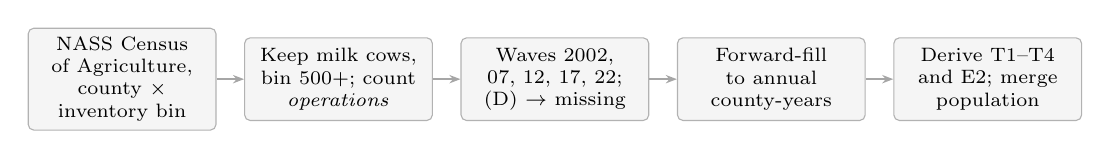
\begin{tikzpicture}[node distance=0.35cm and 0.35cm,
  box/.style={draw=gray!60, rounded corners=2pt, fill=gray!8, align=center, font=\scriptsize, minimum height=1.05cm, text width=2.15cm},
  arr/.style={-{Stealth[length=4pt]}, gray!70, thick}]
\node[box] (a) {NASS Census of Agriculture, county $\times$ inventory bin};
\node[box, right=of a] (b) {Keep milk cows, bin 500$+$; count \emph{operations}};
\node[box, right=of b] (c) {Waves 2002, 07, 12, 17, 22; (D) $\rightarrow$ missing};
\node[box, right=of c] (d) {Forward-fill to annual county-years};
\node[box, right=of d] (e) {Derive T1--T4 and E2; merge population};
\draw[arr] (a) -- (b); \draw[arr] (b) -- (c); \draw[arr] (c) -- (d); \draw[arr] (d) -- (e);
\end{tikzpicture}
\end{center}
\vspace{0.4em}
{\footnotesize
\textbf{Operations, not head.} \emph{Head} is total inventory in the bin. \emph{Operations} is the number of farms. The count uses operations; head$\,\div\,$operations gives average herd size only.\\[0.3em]
\textbf{No zero-filling.} Treatment is missing wherever the NASS cell is suppressed (D).\\[0.3em]
\textbf{Rural sample.} Urban counties are dropped using the NCHS urban--rural classification.\\[0.3em]
\textbf{Consequence of forward-filling.} Every within-county change occurs at a wave year. Timing inside a five-year window is not observed.}
\end{frame}

\begin{frame}{Timing of treatment variation}
\begin{columns}[T,onlytextwidth]
\column{0.42\textwidth}
\begin{center}\footnotesize
\begin{tabular}{lr}
\toprule
Wave & Counties changing status \\
\midrule
2007 & 163 \\
2012 & 123 \\
2017 & 101 \\
2022 & \phantom{0}89 \\
\bottomrule
\end{tabular}
\end{center}
\column{0.55\textwidth}
{\footnotesize
All within-county variation occurs at these four dates.\\[0.4em]
Treatment timing carries up to five years of measurement error. Event-time coefficients near zero are partly contaminated by already-treated years.\\[0.4em]
A window with no wave transition has no treatment variation: county fixed effects absorb the treatment. This binds on A4 (2017--2023), which contains one transition, 2022.}
\end{columns}
\end{frame}

\begin{frame}{E2 vs T1: worked example, FIPS 01043}
\vspace{-4pt}
\begin{center}\footnotesize
\begin{tabular}{@{}lccl@{}}
\toprule
Years & Large dairy count & T1 & E2 \\
\midrule
2002--2006 & 1 & 1 & \alert{0} \quad {\scriptsize has one, but has not \emph{gained} one} \\
2007--2011 & 0 & 0 & 0 \quad {\scriptsize lost it} \\
2012--2016 & 1 & 1 & \alert{1} \quad {\scriptsize count goes $0\to1$: the gain} \\
2017--2023 & 0 & \alert{0} & \alert{1} \quad {\scriptsize lost it again; E2 stays on} \\
\bottomrule
\end{tabular}
\end{center}
\vspace{0.4em}
{\footnotesize
T1 asks: does the county have a large dairy \emph{right now}? \quad E2 asks: has it \emph{ever gained} one?\\[0.3em]
1. From 2017 this county has no large dairy but is coded treated. If effects fade after closure, E2 dilutes them.\\[0.2em]
2. A county with large dairies throughout that never adds one is coded $0$ and sits in the control group.\\[0.3em]
Counties ever T1$=1$: \textbf{759}. Ever E2$=1$: \textbf{572}. The 187-county difference is in the \emph{control} group.}
\end{frame}

\begin{frame}{E2 cohorts: counties first gaining a large dairy}
\begin{columns}[T,onlytextwidth]
\column{0.50\textwidth}
\tbl[0.5]{tables/tab_cohorts.tex}
\column{0.48\textwidth}
\includegraphics[width=\linewidth]{figs/cohorts.pdf}
\end{columns}
\vspace{0.2em}
{\scriptsize
\textbf{Only E2 has cohorts.} Cohort $g$ is the census wave in which a county first gains a large dairy operation. T1--T4 are levels that can rise and fall, so they define no first-treated year and no cohort.\\[0.2em]
\textbf{Cells} count counties in each outcome's estimation sample whose first gain is in wave $g$. They differ across outcomes because the outcome samples cover different counties and years.\\[0.2em]
\textbf{Dashes:} the cohort's base year $g-1$ falls before the outcome starts, so it has no pre-period (Poor MH Days starts 2010, so the 2007 cohort drops; FMD starts 2016).}
\end{frame}

\begin{frame}{F: slaughterhouse treatment}
\vspace{0pt}{\footnotesize
\textbf{Definition.} $F_{it}=1$ if county $i$ has $\geq 1$ FSIS-registered meat or poultry establishment in year $t$. FSIS data cover 2017--2023.\\[0.5em]
\textbf{Current use.} Interacted with dairy in A4 only.\\[0.5em]
\textbf{As a separate treatment (next run).}
\begin{itemize}\footnotesize
  \item Counties with a plant in 2017 have no pre-period: always-treated, excluded from DiD.
  \item Identification comes from openings in 2018--2023 only, against never- and not-yet-treated counties.
  \item Mental health outcomes run to 2023 and overlap. Crime ends 2021 and despair 2020, so openings after those years add nothing for them.
  \item Smaller sample than dairy; report counties per cohort and the MDE before reading coefficients.
\end{itemize}
\vspace{0.3em}
\textbf{Next step:} build $F$ cohorts from establishment grant dates and tabulate openings by year.}
\end{frame}

% =====================================================================
\section{Control variables ($X_{it}$)}

\begin{frame}{Controls: the step-8 set (as run)}
\vspace{-4pt}
\begin{center}\footnotesize
\begin{tabular}{@{}rllrl@{}}
\toprule
\# & Covariate & Source & Coverage & Next run \\
\midrule
1 & Median household income & SAIPE & 99.9\% & keep \\
2 & Unemployment rate & BLS LAUS & 99.7\% & keep \\
3 & \% 65 and older & Census PEP & 99.9\% & keep \\
4 & \% Hispanic & Census PEP & 99.9\% & relabel Latin(x) \\
5 & \% below 18 & Census PEP & 99.9\% & keep \\
6 & Children in poverty & SAIPE & 99.9\% & keep \\
7 & \% female & Census PEP & 99.9\% & \alert{drop} \\
8 & \% Asian & Census PEP & 99.9\% & combine with NA/PI \\
\bottomrule
\end{tabular}
\end{center}
\vspace{0.3em}
{\footnotesize All eight are annual and re-sourced to their data years, so each can be tested for differential pre-trends. Joint listwise coverage on the headline sample: \textbf{34{,}098 of 34{,}199 rows (99.7\%)}. Recodes are in \S7.}
\end{frame}

\begin{frame}{How the eight were arrived at}
\begin{enumerate}\footnotesize
  \item \textbf{Candidate pool.} Non-identifier, non-treatment, non-outcome columns: 107 (105 numeric).
  \item \textbf{Coverage screen.} $\geq 92\%$ complete on rows with a non-missing outcome $\rightarrow$ 26.
  \item \textbf{Remove mediators.} Health and economic measures a CAFO could move $\rightarrow$ 18.
  \item \textbf{Remove for cause.} Colliders, a spliced series, an unusable series, no non-metro variation.
  \item \textbf{Remove untestable.} Rolling or model-smoothed series whose pre-trends cannot be assessed.
  \item \textbf{Order fixed in advance.} Entered one at a time before any coefficient is read.
\end{enumerate}
\vspace{0.3em}
{\footnotesize Fixing the specification before reading results keeps the reported $p$-values valid. Across the eight steps $\hat\beta$ (T1, Poor MH Days, A2) moves from 0.082 to 0.080: the controls barely affect the estimate, consistent with keeping only essential ones in the main specification.}
\end{frame}

\begin{frame}{Excluded: for cause}
\vspace{-4pt}
\begin{center}\footnotesize
\begin{tabular}{@{}llp{6.4cm}@{}}
\toprule
Variable & Ground & Detail \\
\midrule
\texttt{adult\_smoking} & \alert{Collider} & Caused by both distress and local economic shocks; 2 significant pre-period coefficients \\[0.2em]
\texttt{teen\_births} & \alert{Collider} & Same structure; CHR pools over 7 years with a publication lag \\[0.2em]
\texttt{access\_healthy\_foods} & Measure break & CHR splices v030 into v083 at the 2013 release \\[0.2em]
\texttt{driving\_alone\_to\_work} & No usable series & No consistent measurement; 2011--2023 only \\[0.2em]
\texttt{\%\_nat\_hawaiian/pi} & No variation & Negligible share in non-metro counties \\
\bottomrule
\end{tabular}
\end{center}
\vspace{0.3em}
{\footnotesize Conditioning on a variable caused by both treatment and outcome induces bias. No exclusion here depends on an estimated coefficient.}
\end{frame}

\begin{frame}{Excluded: pre-trends cannot be tested}
\vspace{-4pt}
\begin{center}\footnotesize
\begin{tabular}{@{}llrp{4.2cm}@{}}
\toprule
Variable & Source & Rows lost & Why untestable \\
\midrule
\texttt{some\_college} & ACS 5-year & 2{,}336 & Rolling 5-year window \\
\texttt{single\_parent\_hh} & ACS 5-year & 2{,}336 & Rolling 5-year window \\
\texttt{not\_prof\_english} & ACS 5-year & 2{,}336 & Rolling 5-year window \\
\texttt{adult\_obesity} & BRFSS & 0 & Model-based estimate, 3-year lag \\
\texttt{uninsured\_adults} & SAHIE & 0 & Begins 2008; plausible mediator \\
\bottomrule
\end{tabular}
\end{center}
\vspace{0.3em}
{\footnotesize A rolling or model-smoothed series cannot show a differential pre-trend whether or not one exists.\\[0.2em]
\texttt{uninsured\_adults} is deferred (Sept 30): a mental-health confounder, but plausibly moved by CAFO employment.}
\end{frame}

\begin{frame}{Variance inflation factors}
\begin{columns}[T,onlytextwidth]
\column{0.5\textwidth}
\begin{center}\scriptsize
\begin{tabular}{@{}lrr@{}}
\toprule
Covariate & Levels (A1) & Within (A2) \\
\midrule
Median HH income & 2.98 & 1.16 \\
Children in poverty & 2.86 & 1.13 \\
\% 65 and older & 2.32 & 1.45 \\
\% below 18 & 2.41 & 1.44 \\
\midrule
Block maximum & 2.98 & 1.45 \\
\bottomrule
\end{tabular}
\end{center}
\column{0.48\textwidth}
\begin{center}\scriptsize
\begin{tabular}{@{}lrrr@{}}
\toprule
Model & Specs & Max VIF & $>10$ \\
\midrule
A1 & 35 & 3.24 & 0 \\
A2 & 35 & 2.39 & 0 \\
A4 & 28 & 3.96 & 0 \\
A5 & 7 & 2.32 & 0 \\
\bottomrule
\end{tabular}
\end{center}
\end{columns}
\vspace{0.5em}
{\footnotesize VIF is computed per model on the design matrix that produced the coefficient. Collinearity among the controls is cross-sectional; county fixed effects remove most of it. No specification has a VIF above 4.}
\end{frame}

% =====================================================================
\section{Outcomes ($Y_{it}$)}

\begin{frame}{$Y_{it}$: outcome variables and units}
\vspace{-6pt}
\begin{center}
\adjustbox{max width=\textwidth, max totalheight=0.55\textheight}{%
\begin{tabular}{@{}llllrr@{}}
\toprule
Outcome & Unit & Source & Years & Mean & SD \\
\midrule
Poor MH Days & Mean days in past 30 & CHR (BRFSS) & 2010--23 & 3.96 & 0.98 \\
Freq.\ Mental Distress & Per 100{,}000 adults & CHR (BRFSS) & 2016--23 & 13{,}544 & 2{,}793 \\
Deaths of Despair & Crude deaths per 100{,}000 & CDC WONDER & 2000--20 & 20.36 & 9.79 \\
Agg.\ Assault & Arrests per 100{,}000 & NIBRS & 2000--21 & 57.05 & 65.78 \\
Assault, all sev. & Arrests per 100{,}000 & NIBRS & 2000--21 & 267.57 & 242.54 \\
Violence (partial) & Arrests per 100{,}000 & NIBRS & 2000--21 & 85.59 & 88.64 \\
NIBRS total & Arrests per 100{,}000 & NIBRS & 2000--21 & 309.94 & 271.38 \\
\bottomrule
\end{tabular}}
\end{center}
{\tiny \textit{Poor MH Days} is a mean: $\beta=0.08$ is 0.08 additional poor-mental-health days per person per 30 days. The rest are per-100{,}000 rates.\\
\alert{NIBRS measures are arrests, not offences}; they also reflect policing intensity. \textit{Assault, all severities} is 79\% simple assault. \textit{Violence (partial)} omits robbery and homicide and is not the UCR violent-crime definition. \textit{NIBRS total} sums 12 person-directed offence types.}
\end{frame}

% =====================================================================
\section{Model results}

\begin{frame}{A1: pooled cross-section (state $+$ year FE)}
\vspace{-4pt}
$$Y_{it} = \beta D_{it} + X_{it}\gamma + \alpha_{s(i)} + \delta_t + \varepsilon_{it}$$
{\footnotesize \textbf{Identifying variation.} Between-county differences within a state-year. Counties are compared to other counties, not to themselves. Step-8 controls; SE clustered by state.}
\vspace{0.6em}
\begin{columns}[T,onlytextwidth]
\column{0.32\textwidth}\textbf{\footnotesize Supporting literature}\\[0.3em]{\footnotesize\textcolor{gray}{\textit{[to add]}}}
\column{0.32\textwidth}\textbf{\footnotesize What we capture}\\[0.3em]{\footnotesize\textcolor{gray}{\textit{[to add]}}}
\column{0.32\textwidth}\textbf{\footnotesize What we lose}\\[0.3em]{\footnotesize\textcolor{gray}{\textit{[to add]}}}
\end{columns}
\end{frame}

\begin{frame}{A1: pooled cross-section, results (T1--T3)}
\vspace{-6pt}
\tbl[0.68]{tables/tab_A1_p1.tex}
\tabnote{Each cell is a separate regression. Step-8 controls; state-clustered SE in parentheses. \starnote.}
\end{frame}

\begin{frame}{A1: pooled cross-section, results (T4, E2)}
\vspace{-6pt}
\tbl[0.68]{tables/tab_A1_p2.tex}
\tabnote{Each cell is a separate regression. Step-8 controls; state-clustered SE in parentheses. \starnote.}
\end{frame}

\begin{frame}{A1: variance inflation factors}
\vspace{-6pt}
\tbl[0.6]{tables/tab_vif_A1.tex}
\tabnote{Each cell is one specification: maximum VIF across all regressors, with the VIF on the treatment in parentheses. Computed on the design matrix that produced the coefficient (raw levels, state FE). No VIF exceeds 10.}
\end{frame}

\begin{frame}{A1: coefficient plot}
\vspace{-6pt}
\begin{center}\includegraphics[width=\textwidth]{figs/coef_A1.pdf}\end{center}
\tabnote{Same construction as the A2 plot. Under state FE the sign reverses for crime and despair: between-county differences dominate, and counties with large dairies have lower levels of these outcomes.}
\end{frame}

\begin{frame}{A2: two-way fixed effects (county $+$ year FE)}
\vspace{-4pt}
$$Y_{it} = \beta D_{it} + X_{it}\gamma + \alpha_i + \delta_t + \varepsilon_{it}$$
{\footnotesize \textbf{Identifying variation.} Within-county changes in treatment, net of nationwide year shocks. Only switching counties identify $\beta$; assumes parallel trends conditional on $X$. Step-8 controls; SE clustered by state.}
\vspace{0.6em}
\begin{columns}[T,onlytextwidth]
\column{0.32\textwidth}\textbf{\footnotesize Supporting literature}\\[0.3em]{\footnotesize\textcolor{gray}{\textit{[to add]}}}
\column{0.32\textwidth}\textbf{\footnotesize What we capture}\\[0.3em]{\footnotesize\textcolor{gray}{\textit{[to add]}}}
\column{0.32\textwidth}\textbf{\footnotesize What we lose}\\[0.3em]{\footnotesize\textcolor{gray}{\textit{[to add]}}}
\end{columns}
\end{frame}

\begin{frame}{A2: two-way fixed effects, results (T1--T3)}
\vspace{-6pt}
\tbl[0.68]{tables/tab_A2_p1.tex}
\tabnote{Each cell is a separate regression. Step-8 controls; state-clustered SE in parentheses. Only switching counties identify $\beta$. \starnote.}
\end{frame}

\begin{frame}{A2: two-way fixed effects, results (T4, E2)}
\vspace{-6pt}
\tbl[0.68]{tables/tab_A2_p2.tex}
\tabnote{Each cell is a separate regression. Step-8 controls; state-clustered SE in parentheses. Only switching counties identify $\beta$. \starnote.}
\end{frame}

\begin{frame}{A2: variance inflation factors}
\vspace{-6pt}
\tbl[0.6]{tables/tab_vif_A2.tex}
\tabnote{Each cell is one specification: maximum VIF across all regressors, with the VIF on the treatment in parentheses. Computed on the design matrix that produced the coefficient (within-transformed, county FE). No VIF exceeds 10.}
\end{frame}

\begin{frame}{A2: coefficient plot}
\vspace{-6pt}
\begin{center}\includegraphics[width=\textwidth]{figs/coef_A2.pdf}\end{center}
\tabnote{$\hat\beta$ divided by the within-county SD of each outcome, so effects are comparable across outcomes within a treatment (not across treatments: units of $D$ differ). Thick bar $\pm1$ SE, thin bar 95\% CI, state-clustered. Darker $=$ more significant.}
\end{frame}






\begin{frame}{A4: dairy $\times$ slaughterhouse}
\vspace{-4pt}
$$Y_{it} = \beta_1 D_{it} + \beta_2 F_{it} + \beta_3 (D \times F)_{it} + X_{it}\gamma + \alpha_i + \delta_t + \varepsilon_{it}$$
{\footnotesize \textbf{Identifying variation.} Within-county changes in dairy, 2017--2023, allowed to differ by slaughterhouse presence. One wave transition (2022) in the window: 89 switchers for the mental health outcomes; crime and despair are not identified.}
\vspace{0.6em}
\begin{columns}[T,onlytextwidth]
\column{0.32\textwidth}\textbf{\footnotesize Supporting literature}\\[0.3em]{\footnotesize\textcolor{gray}{\textit{[to add]}}}
\column{0.32\textwidth}\textbf{\footnotesize What we capture}\\[0.3em]{\footnotesize\textcolor{gray}{\textit{[to add]}}}
\column{0.32\textwidth}\textbf{\footnotesize What we lose}\\[0.3em]{\footnotesize\textcolor{gray}{\textit{[to add]}}}
\end{columns}
\end{frame}

\begin{frame}{A4: dairy $\times$ slaughterhouse, results}
\vspace{-6pt}
\tbl[0.6]{tables/tab_A4.tex}
{\scriptsize \textbf{Reading:} $\beta_1\approx0$ and $\beta_3>0$ for Poor MH Days: the dairy association is concentrated in counties that also have a plant.}\\
\tabnote{State-clustered SE in parentheses; for $\beta_1,\beta_2$ recovered from saved $p$-values ($t$, $G-1$ df). \starnote.}
\end{frame}

\begin{frame}{A4: variance inflation factors}
\vspace{-6pt}
\tbl[0.6]{tables/tab_vif_A4.tex}
\tabnote{Each cell is one specification: maximum VIF across all regressors, with the VIF on the treatment in parentheses. Computed on the design matrix that produced the coefficient. The maximum is the $D\times F$ interaction in every column, which is expected: it is built from $D$.}
\end{frame}

\begin{frame}{A5: event study}
\vspace{-4pt}
$$Y_{it} = \sum_{e \neq -1} \theta_e\, \mathbb{1}[t - g_i = e] + X_{it}\gamma + \alpha_i + \delta_t + \varepsilon_{it}$$
{\footnotesize \textbf{Identifying variation.} Outcome paths before and after a county's first gain ($g_i$, E2), relative to $e=-1$. Leads ($e<-1$) are the placebo test. County $+$ year FE, step-8 controls, $\pm8$ years, state-clustered SE.}
\vspace{0.6em}
\begin{columns}[T,onlytextwidth]
\column{0.32\textwidth}\textbf{\footnotesize Supporting literature}\\[0.3em]{\footnotesize\textcolor{gray}{\textit{[to add]}}}
\column{0.32\textwidth}\textbf{\footnotesize What we capture}\\[0.3em]{\footnotesize\textcolor{gray}{\textit{[to add]}}}
\column{0.32\textwidth}\textbf{\footnotesize What we lose}\\[0.3em]{\footnotesize\textcolor{gray}{\textit{[to add]}}}
\end{columns}
\end{frame}

\begin{frame}{A5: event studies, mental health and mortality}
\vspace{-6pt}
\begin{center}\includegraphics[width=\textwidth]{figs/es_mental.pdf}\end{center}
\tabnote{Coefficients in outcome units, 95\% CI, state-clustered. Pre-period points shaded by significance. No pre-period coefficient is significant at 5\% for these three outcomes.}
\end{frame}

\begin{frame}{A5: event studies, crime}
\vspace{-6pt}
\begin{center}\includegraphics[width=\textwidth]{figs/es_crime.pdf}\end{center}
\tabnote{Coefficients in outcome units, 95\% CI, state-clustered. Pre-period points shaded by significance.}
\end{frame}

\begin{frame}{A5: pre-trend test}
\begin{columns}[T,onlytextwidth]
\column{0.55\textwidth}
\tbl[0.55]{tables/tab_A5_pretrend.tex}
\column{0.43\textwidth}
{\footnotesize
\textbf{Crime fails.} Aggravated assault, all assault and the NIBRS total each have 2--3 significant pre-period coefficients. Treated counties were already on different arrest trajectories.\\[0.4em]
Per Sept 30, these pre-trends are disqualifying for the crime outcomes under the current design.\\[0.4em]
Mental health and mortality outcomes are flat.}
\end{columns}
\end{frame}

\begin{frame}{A5: variance inflation factors}
\vspace{-6pt}
\tbl[0.6]{tables/tab_vif_A5.tex}
\tabnote{Maximum VIF over the covariate block. The event-time indicators partition the sample and are collinear by construction, so they are excluded.}
\end{frame}

\begin{frame}{A6: Callaway--Sant'Anna}
\vspace{-4pt}
$$\mathrm{ATT}(g,t) = \mathbb{E}\!\left[Y_t - Y_{g-1} \mid G = g\right] - \mathbb{E}\!\left[Y_t - Y_{g-1} \mid \text{not yet / never treated}\right]$$
{\footnotesize \textbf{Identifying variation.} Long differences from $g-1$ for each cohort against counties not yet treated at $t$ or never treated; no already-treated controls. Aggregated by cohort size; 300-rep state cluster bootstrap. Unconditional and covariate-adjusted arms. No VIF: estimates cell means, not a regression.}
\vspace{0.6em}
\begin{columns}[T,onlytextwidth]
\column{0.32\textwidth}\textbf{\footnotesize Supporting literature}\\[0.3em]{\footnotesize\textcolor{gray}{\textit{[to add]}}}
\column{0.32\textwidth}\textbf{\footnotesize What we capture}\\[0.3em]{\footnotesize\textcolor{gray}{\textit{[to add]}}}
\column{0.32\textwidth}\textbf{\footnotesize What we lose}\\[0.3em]{\footnotesize\textcolor{gray}{\textit{[to add]}}}
\end{columns}
\end{frame}

\begin{frame}{A6: Callaway--Sant'Anna, results}
\vspace{-6pt}
\tbl[0.6]{tables/tab_A6.tex}
\tabnote{All rows use E2, so only the estimator varies. SE in parentheses: state-clustered (TWFE), 300-rep state cluster bootstrap (CS). \starnote.}
\end{frame}

% =====================================================================
\section{Comparing model runs}

\begin{frame}{TWFE vs Callaway--Sant'Anna}
\vspace{-6pt}
\begin{center}\includegraphics[width=\textwidth,height=0.6\textheight,keepaspectratio]{figs/twfe_vs_cs.pdf}\end{center}
\tabnote{Same treatment (E2) throughout. CS estimates are smaller than TWFE for every outcome except Deaths of Despair (null in both). The gap is the share of the TWFE estimate that comes from already-treated counties serving as controls. Only Frequent Mental Distress (CS unconditional) stays significant at 5\%.}
\end{frame}

\begin{frame}{Effect size against the minimum detectable effect: E2}
\vspace{-6pt}
\tbl[0.55]{tables/tab_mde_E2.tex}
\tabnote{County $+$ year FE, step-8 controls, state-clustered SE. $\hat\beta/\sigma_w$ is the coefficient in within-county SDs of the outcome, placed next to MDE$_{\sigma_w}$ $=2.80\times$SE$/\sigma_w$ (80\% power, two-sided $\alpha=0.05$). Bold: $|\hat\beta/\sigma_w|\geq$ MDE. \starnote.}
\end{frame}

\begin{frame}{Effect size against the minimum detectable effect: T1}
\vspace{-6pt}
\tbl[0.55]{tables/tab_mde_T1.tex}
\tabnote{As previous slide, treatment T1 (presence). Crime MDEs are about one-third of a within-county SD: the design can detect only large crime effects. Other treatments in the appendix.}
\end{frame}

\begin{frame}{Stability of $\hat\beta$ as controls are added}
\vspace{-6pt}
\tbl[0.5]{tables/tab_stability.tex}
\tabnote{Each path is one FE $\times$ outcome $\times$ treatment combination (56). Median $|\Delta\beta|$: median absolute \% change in the coefficient from the treatment-only model to the full control sequence. Within (county) FE halves fragility relative to pooled; log(1$+$count) is the most stable treatment; per-capita is the least.}
\end{frame}

\begin{frame}{Standard errors: clustering choice (A2, E2)}
\vspace{-6pt}
\tbl[0.55]{tables/tab_se_compare.tex}
\tabnote{Same point estimate under three variance estimators. State clustering (48 clusters) is the most conservative and is the reported default. \starnote.}
\end{frame}

% =====================================================================
\section{Robustness: spatial spillovers}

\begin{frame}{Spatial spillovers: five checks}
\vspace{-6pt}
{\footnotesize
If neighbouring counties share outcomes or are reached by a nearby dairy, near-by never-treated counties are not clean controls and state-clustered standard errors may be too small. Five checks on the reported set:}
\vspace{0.1em}
\begin{center}\scriptsize
\begin{tabular}{@{}rp{3.0cm}p{8.2cm}@{}}
\toprule
 & Check & What it does \\
\midrule
1 & Moran's I & Spatial correlation of the outcome and of the A2 residual, by year (counties within 100 km; 499 permutations). \\[0.05em]
2 & Donut comparison group & Drop never-treated counties within 50 or 100 km of a treated county; re-estimate TWFE and Callaway--Sant'Anna. \\[0.05em]
3 & Conley standard errors & Allow correlation between counties within 250 km; compared with state clustering on the 28 A2 cells. \\[0.05em]
4 & Division $\times$ year effects & Replace year effects with Census-division-by-year effects (nine divisions) in the A2 cells. \\[0.05em]
5 & Spatial Durbin model & Outcome depends on neighbours' outcomes and neighbours' treatment; direct, indirect and total effects. \\
\bottomrule
\end{tabular}
\end{center}
\end{frame}

\begin{frame}{Spatial Durbin model: specification}
\vspace{-4pt}
$$Y_{it} = \rho \sum_j w_{ij} Y_{jt} + \beta D_{it} + \theta \sum_j w_{ij} D_{jt} + X_{it}\gamma + \alpha_i + \delta_t + \varepsilon_{it}$$
{\footnotesize
\textbf{Neighbours.} $w_{ij}$: counties whose centroids are within 100 km, row-standardised, panel counties only.\\[0.3em]
\textbf{Terms.} $\rho$: dependence of a county's outcome on its neighbours' outcomes. $\theta$: effect of neighbours' treatment. The neighbour average enters for the treatment only, not for the controls.\\[0.3em]
\textbf{Effects.} Direct, indirect (spillover) and total effects, in outcome units; maximum likelihood with simulation standard errors, and a state-block wild bootstrap (499 draws) for the confirmatory family.\\[0.3em]
\textbf{Sample.} Balanced panel of the counties observed in every year of the outcome's window. A TWFE-type model, so not robust to staggered timing.\\[0.3em]
Commuting-zone weights are also run (not shown). Panel 2026-10-25.}
\end{frame}

\begin{frame}{Spillovers: spatial correlation (Moran's I)}
\input{generated/robust__spill_moran.tex}
\end{frame}

\begin{frame}{Spillovers: dropping nearby comparison counties, E2}
\begin{center}
\includegraphics[width=\textwidth,height=0.70\textheight,keepaspectratio]{generated/assets/forest_donut_first_expansion__main.pdf}
\end{center}
\vspace{-4pt}
{\tiny\baselineskip=6.5pt Estimate with 95\% interval in within-county SD of the outcome, as never-treated comparison counties within 50 and 100 km of a treated county are dropped; TWFE and covariate-adjusted Callaway-Sant'Anna (not-yet-treated counties stay in its comparison group). Panel 2026-10-25; standard errors clustered by state (Callaway-Sant'Anna: state bootstrap).\par}
\end{frame}

\begin{frame}{Spillovers: dropping nearby comparison counties, E3}
\begin{center}
\includegraphics[width=\textwidth,height=0.70\textheight,keepaspectratio]{generated/assets/forest_donut_first_entry__main.pdf}
\end{center}
\vspace{-4pt}
{\tiny\baselineskip=6.5pt Estimate with 95\% interval in within-county SD of the outcome, as never-treated comparison counties within 50 and 100 km of a treated county are dropped; TWFE and covariate-adjusted Callaway-Sant'Anna (not-yet-treated counties stay in its comparison group). Panel 2026-10-25; standard errors clustered by state (Callaway-Sant'Anna: state bootstrap).\par}
\end{frame}

\begin{frame}{Spillovers: dropping nearby comparison counties, T1, T3, T4}
\begin{center}
\includegraphics[width=\textwidth,height=0.70\textheight,keepaspectratio]{generated/assets/forest_donut_dose__main.pdf}
\end{center}
\vspace{-4pt}
{\tiny\baselineskip=6.5pt Estimate with 95\% interval in within-county SD of the outcome, as never-treated comparison counties within 50 and 100 km of a treated county are dropped; TWFE; a comparison county is one that is never positive on the treatment. Panel 2026-10-25; standard errors clustered by state (Callaway-Sant'Anna: state bootstrap).\par}
\end{frame}

\begin{frame}{Spillovers: standard errors (state-clustered and Conley)}
\input{generated/robust__spill_conley.tex}
\end{frame}

\begin{frame}{Spillovers: division-by-year fixed effects}
\input{generated/robust__spill_division.tex}
\end{frame}

\begin{frame}{Spillovers: spatial Durbin model, sample and spatial dependence}
\input{generated/robust__spill_durbin_sample.tex}
\end{frame}

\begin{frame}{Spillovers: spatial Durbin model, direct and spillover effects}
\begin{center}
\includegraphics[width=\textwidth,height=0.70\textheight,keepaspectratio]{generated/assets/forest_durbin__main.pdf}
\end{center}
\vspace{-4pt}
{\tiny\baselineskip=6.5pt Spatial Durbin panel model, county and year effects, weights: counties within 100 km; balanced panel of the counties observed in every year of the outcome's window. Effects in within-county SD; 95\% intervals from maximum-likelihood simulation standard errors (the bootstrap is in the table on the next page). A TWFE-type model, not robust to staggered timing. Panel 2026-10-25.\par}
\end{frame}

\begin{frame}{Spillovers: spatial Durbin model, bootstrap check}
\input{generated/robust__spill_durbin_boot.tex}
\end{frame}

% =====================================================================
\section{Next steps}

\begin{frame}{Next step: nearest-neighbour Gaussian process (NN-RCM)}
\vspace{-4pt}
\begin{columns}[T,onlytextwidth]
\column{0.48\textwidth}
{\footnotesize
\textbf{What it is.} \texttt{NNRCM}, an R package (C++ core) for spatial inference and prediction with the univariate and bivariate nearest-neighbour Gaussian process with a random covariance matrix (NN-RCM).
\begin{itemize}\footnotesize
  \item Spatial dependence may vary by location (non-stationary) and by direction (non-isotropic).
  \item Each location conditions on a few nearest neighbours, so large spatial data sets are feasible.
  \item Estimation by MCMC, or by marginal-likelihood maximisation (faster for large data).
\end{itemize}}
\column{0.50\textwidth}
{\footnotesize
\textbf{Why here.} The checks above use one fixed neighbour rule (100 km) and, in the Durbin model, one dependence parameter $\rho$ for the whole country. NN-RCM is a model-based alternative that lets dependence differ across space.\\[0.5em]
\textbf{Candidate use (not yet specified).} Fit the model to county-level residuals from the A2 regression at county centroids (outlines are in hand) and ask whether the spatial structure changes the treatment estimate or its uncertainty.}
\end{columns}
\end{frame}

\begin{frame}{NN-RCM: open questions before a run}
\vspace{0pt}{\footnotesize
\textbf{Not yet confirmed.}
\begin{itemize}\footnotesize
  \item Whether the package accepts county-year panel data and fixed effects, or only one cross-section of locations at a time.
  \item What it needs as input (county centroids are available) and how a treatment effect, rather than a spatial prediction, is recovered from it.
\end{itemize}
\vspace{0.3em}
\textbf{Source of the description.} The package's own \texttt{DESCRIPTION} file and file names; the package page has no README. No accompanying paper or vignette has been read yet.\\[0.5em]
\textbf{Before any run.} Read the vignette and the source paper; write a plan and a decision-register entry (it touches the spatial specification).}
\end{frame}

\begin{frame}{Population and the event-study pre-trends}
\vspace{0pt}{\footnotesize
\textbf{What is already absorbed.} A5 includes county FE, so any time-invariant county trait is gone, including land area. Within a county, $\log(\text{density}) = \log(\text{pop}) - \log(\text{area})$, so density and log population are the same control once county FE are in.\\[0.5em]
\textbf{What is not.} Time-varying population. Two channels matter here:
\begin{itemize}\footnotesize
  \item Outcomes are per-100{,}000 rates, so population is the denominator. Counties losing population mechanically raise their rates.
  \item Large dairies may enter counties that are depopulating, which would generate the crime pre-trends without any CAFO effect.
\end{itemize}
\vspace{0.3em}
\textbf{But population is a candidate bad control:} CAFO employment can move it after entry.\\[0.5em]
\textbf{Plan.} (1) Event study with $\log$ population as the \emph{outcome}: a direct test of differential depopulation. (2) Re-estimate A5 with $\log$ population measured at $g-1$, interacted with year, so it adjusts for pre-entry trends without conditioning on post-entry population.}
\end{frame}

\begin{frame}{Slaughterhouse as treatment: design}
\vspace{0pt}{\footnotesize
\begin{itemize}\footnotesize
  \item Treatment: first year with an FSIS establishment ($F$ cohorts 2018--2023)
  \item Estimator: CS, same controls and inference as dairy
  \item Outcomes: Poor MH Days and Frequent Mental Distress (overlap through 2023); crime and despair only for openings by 2020--21
  \item Report first: openings by year, counties per cohort, MDE
  \item Separate species: meat vs poultry slaughter grants
\end{itemize}
\vspace{0.4em}
A4 suggests the dairy association for Poor MH Days runs through counties with plants. A standalone $F$ estimate tests whether plants matter without dairy.}
\end{frame}

% =====================================================================
\section{Future changes: demographics}

\begin{frame}{Demographic controls: changes for the next run}
\vspace{-4pt}
\begin{center}\scriptsize
\begin{tabular}{@{}p{3.6cm}p{3.4cm}p{6.2cm}@{}}
\toprule
Variable & Change & Reason \\
\midrule
\% female & Drop & Little within-county variation; adds variance, not adjustment \\
\% Asian, \% Native American, \% PI & Combine into one group & Small non-metro shares; NA/PI alone has no variation \\
\% Hispanic & Relabel Latin(x) & Census PEP category is Hispanic or Latino; label only \\
\% Black, \% Native American & Include & State the full racial composition used \\
Reference group & \% non-Hispanic white omitted & Shares sum to one; one category must be omitted \\
\bottomrule
\end{tabular}
\end{center}
\vspace{0.3em}
{\footnotesize Already applied: teen births removed (collider). Deferred: uninsured adults. Each change is re-tested for pre-trends and re-run through the VIF audit before results are read.}
\end{frame}

\begin{frame}{Demographic-specific outcomes (longer run)}
\begin{itemize}\footnotesize
  \item \textbf{Frequent Mental Distress by sex.} Check CHR/BRFSS subgroup availability; a sex-specific outcome removes composition noise from the county mean.
  \item \textbf{Outcomes by race and ethnicity.} CDC WONDER mortality is already downloaded by race $\times$ gender (ages 15--65). CHR survey measures need a subgroup source.
  \item \textbf{Demographic-specific panel.} County $\times$ group $\times$ year, built downstream in code, not as a new merged dataset.
  \item \textbf{Order.} Heterogeneity is estimated only if an aggregate effect survives CS; otherwise subgroup results multiply tests without a prior.
\end{itemize}
\end{frame}

% =====================================================================

\begin{frame}{Appendix: effect size against MDE, T2}
\vspace{-6pt}\tbl[0.55]{tables/tab_mde_T2.tex}
\tabnote{County $+$ year FE, step-8 controls, state-clustered SE. Bold: $|\hat\beta/\sigma_w|\geq$ MDE$_{\sigma_w}$. \starnote.}
\end{frame}
\begin{frame}{Appendix: effect size against MDE, T3}
\vspace{-6pt}\tbl[0.55]{tables/tab_mde_T3.tex}
\tabnote{As above, treatment T3 (per 10{,}000 residents). \starnote.}
\end{frame}
\begin{frame}{Appendix: effect size against MDE, T4}
\vspace{-6pt}\tbl[0.55]{tables/tab_mde_T4.tex}
\tabnote{As above, treatment T4 ($\log(1+\text{count})$). \starnote.}
\end{frame}

\end{document}
